\chapter{Атом гелия}

\section{Атом гелия. Спиновые функции двух электронов. Пара- и ортосостояния}

Атом гелия --- простейшая многочастичная система, содержащая тождественные частицы. Кроме того, атом He --- самый простой из сложных атомов. Эти два аргумента объясняют то внимание, которое мы уделяем решению задачи об атоме гелия (см. \autoref{fig:17_1}).
\begin{figure}[h!]
\centering
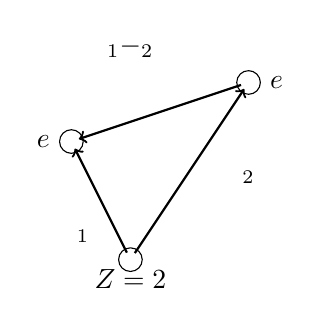
\begin{tikzpicture}[domain=-3:3, scale = 1.5]
  \node [below] at (0, 0) {$Z=2$};  
  \draw (0, 0) circle (1mm);  
  \draw (-0.5, 1) circle (1mm);
  \node [left] at (-0.6, 1) {$e$};  
  \draw (1, 1.5) circle (1mm);
  \node [right] at (1.1, 1.5) {$e$};  
  \draw[<-, thick, shorten >=1mm, shorten <= 1mm] (-0.5, 1) -- (0, 0);
  \node at (-0.4, 0.2) {$\vr_1$};
  \draw[<-,thick, shorten >=1mm, shorten <= 1mm] (1, 1.5) -- (0, 0);
  \node at (1, 0.7) {$\vr_2$};
  \draw[<-,thick, shorten >=1mm, shorten <= 1mm] (-0.5, 1) -- (1, 1.5);
   \node at (0, 1.8) {$\vr_1 - \vr_2$};
\end{tikzpicture}
\caption{Атом гелия.} \label{fig:17_1}
\end{figure}

Гамильтониан системы (два тождественных электрона в поле точечного ядра) имеет вид:
\begin{equation}
\label{eq:17_1_1}
\op{H} = \frac{\op{\vp}_1^2}{2m} - \frac{Ze^2}{r_1} + \frac{\op{\vp}_2^2}{2m} - \frac{Ze^2}{r_2} + \frac{e^2}{\abs{\vr_1 - \vr_2}}
\end{equation}

Здесь для атома гелия порядковый номер ядра $Z = 2$. Необходимо решить стационарное уравнение Шрёдингера
\begin{equation}
\label{eq:17_1_2}
\op{H} \Psis(\xi_1, \xi_2) =E\Psis(\xi_1, \xi_2),
\end{equation}
то есть определить уровни энергии и состояние двух электронов в атоме He.

Заметим, что в нерелятивистском приближении спиновые эффекты (спин-орбитальное взаимодействие) возникают в порядке $\brc{\dfrac{v}{c}}^2 \ll 1$ (см. \S 4 главы \rom{14}). Если спин-орбитальное взаимодействие не учитывать, то взаимодействие от спина не зависит. Поскольку гамильтониан $\op{H}$ не содержит спиновых операторов, то в полном решении координатные и спиновые функции разделяются:
$$
\Psis(\xi_1, \xi_2) = \Phi(\vr_1, \vr_2) \chi(\sigma_1, \sigma_2)
$$

Согласно введенному в \S 1 главы \rom{16} постулату о тождественных частицах, полная волновая функция (т.~е. с учетом спиновых переменных) должна быть антисимметричной к перестановке частиц, т.~к. электроны --- это фермионы. Поэтому возможны два решения:
$$
\Psis_1 = \Phi^S(\vr_1, \vr_2) \chi^A(\sigma_1, \sigma_2)
$$
$$
\Psis_2 = \Phi^A(\vr_1, \vr_2) \chi^S(\sigma_1, \sigma_2)
$$

В соответствии с правилом сложения моментов \eqref{eq:15_2_4}, собственные значения суммарного спинового момента двух электронов $s = 0, 1$.

Тогда собственными векторами операторов $\op{\vec{s}}_1^2$, $\op{\vec{s}}_2^2$, $\op{\vec{s}}^2$, $\op{s}_z$ являются $\ket{s s_z}$, где $s = 0$, $s_z = 0$; $s = 1$, $s_z=-1, 0, 1$.

Нетрудно найти собственные функции системы из двух частиц со спинами $\dfrac{1}{2}$:
$$
\chi(0, 0) = \frac{1}{\sqrt{2}}\brc{\alpha(1)\beta(2) - \beta(1)\alpha(2)}
$$
--- синглетная <<S>> спиновая волновая функция.

\begin{gather*}
\chi(1, 1) = \alpha(1)\alpha(2) \\
\chi(1, 0) = \frac{1}{\sqrt{2}}\brc{\alpha(1)\beta(2) + \beta(1)\alpha(2)} \\
\chi(1, -1) = \beta(1)\beta(2)
\end{gather*}
--- триплетная <<T>> спиновая волновая функция.

Легко видеть, что функция $\chi^S(\sigma_1, \sigma_2)$ \underline{симметрична} относительно перестановки спиновых переменных, если $s = 1$, а функция $\chi^A(\sigma_1, \sigma_2)$ \underline{антисимметрична}, если $s = 0$.

Таким образом, состояния атома He можно классифицировать по значению суммарного спина электронов: $s = 0$ --- парагелий (синглетные уровни), $s = 1$ --- ортогелий (триплетные уровни).

Интересно, что оба вида атомов ведут себя независимо с точки зрения процессов излучения. Электрические дипольные переходы с $\Delta s \neq 0$ запрещены. Поэтому запрещены и дипольные переходы из одного состояния в другое. Фактически, спектральные линии отвечают смеси двух индивидуальных <<веществ>>.

\section{Обменное взаимодействие}

В качестве первого шага решения двухэлектронной задачи \eqref{eq:17_1_2} воспользуемся стационарной теорией возмущений. Для этого представим гамильтониан системы He в виде суммы
$$
\op{H} = \op{H}^\zr + \op{V}
$$

гамильтониана $\op{H}^\zr$ двух невзаимодействующих друг с другом электронов $\op{H}^\zr = \op{H}_1 + \op{H}_2$, где $\op{H}_i = \dfrac{\op{\vp_i}^2}{2m} - \dfrac{Ze^2}{r_i}$ и оператора $\op{V}$ межэлектронного отталкивания
$$
\op{V} = \frac{e^2}{\abs{\vr_1 - \vr_2}},
$$
рассматриваемого как возмущение. В нулевом приближении имеем обычные водородоподобные функции независимых электронов, а волновая функция $\Psis(\xi_1, \xi_2)$ всей системы должна строиться как их правильная антисимметризованная комбинация.

Пусть эти электроны находятся в пространственных состояниях $\nu_1$ (квантовые числа $n_1$, $l_1$, $m_1$) и $\nu_2$ (квантовые числа $n_2$, $l_2$, $m_2$). С учетом результатов предыдущего параграфа \underline{правильную} к перестановке координат $\vr_1$ и $\vr_2$ пространственную волновую функцию можно записать в виде:

%Если $\nu_1 \not = \nu_2$, то такие электроны называются неэквивалентными.

%Если $\nu_1 = \nu_2$, то такие электроны называются эквивалентными.

\begin{eqnarray}
\label{eq:17_2_1}
\Phi^{A, S}(\vr_1, \vr_2) &=& \frac{1}{\sqrt{2}}\brcr{\phi_{\nu_1}(\vr_1) \phi_{\nu_2}(\vr_2) \mp \phi_{\nu_2}(\vr_1) \phi_{\nu_1}(\vr_2)}, ~~~\nu_1 \neq \nu_2 \nonumber \\
\Phi^S(\vr_1, \vr_2) &=& \phi_{\nu}(\vr_1) \phi_{\nu}(\vr_2), ~~~\nu_1 = \nu_2= \nu
\end{eqnarray}

Последняя запись не противоречит принципу Паули, поскольку в антисимметричном спиновом состоянии $\chi(0, 0)$ ($s=0$) электроны находятся в разных квантовых состояниях с противоположными направлениями спина.

Допустимые волновые функции атома He, в соответствии с предыдущим \S 1, есть
\begin{equation}
\label{eq:17_2_2}
\underbrace{\Phi^S \chi(0, 0)}_{s = 0};~~~\underbrace{\Phi^A \chi(1,1),~~~\Phi^A \chi(1,0),~~~\Phi^A \chi(1,-1)}_{s = 1}
\end{equation}

Подчеркнем, что в нулевом приближении все четыре состояния, описываемые функциями \eqref{eq:17_2_2}, \underline{вырождены}. Их энергия равна сумме энергий для состояний $\nu_1$ и $\nu_2$:
$$
E_{\nu_1, \nu_2}^\zr = E_{\nu_1} + E_{\nu_2} \equiv E_{n_1} + E_{n_2}
$$

Найдем теперь энергетическое расщепление состояний \eqref{eq:17_2_2} при учете кулоновского отталкивания между электронами в первом порядке теории возмущений.

Если электроны эквивалентны ($\nu_1 = \nu_2= \nu$), то $\Phi^A \equiv 0$ и возможно лишь синглетное состояние $\Psi^S \chi(0, 0)$, которое сдвигается возмущением ${\op{V} = \dfrac{e^2}{\abs{\vr_1 - \vr_2}}}$. Для неэквивалентных электронов ($\nu_1 \neq \nu_2$) допустимы все четыре функции \eqref{eq:17_2_2}. Поскольку $\op{V}$ не зависит от спинов, триплетные состояния останутся вырожденными.

Однако синглет и триплет теперь расщепляются: хотя силы межэлектронного кулоновского отталкивания не зависят от $s$, но $s$ определяет возможную симметрию пространственной волновой функции и тем самым влияет на энергию.

В первом приближении теории возмущений энергетический сдвиг состояний \eqref{eq:17_2_1} с $\nu_1 \neq \nu_2$
\begin{equation}
\label{eq:17_2_3}
\boxed{E_{\nu_1 \nu_2}^\one = \bfk{\Phi^{S, A}}{\op{V}}{\Phi^{S, A}} = J_{\nu_1 \nu_2} \pm K_{\nu_1 \nu_2}},
\end{equation}
где значению $s = 0$ отвечает знак <<+>> , а значению $s = 1$ --- знак <<->>.
\begin{eqnarray}
\label{eq:17_2_4}
J_{\nu_1 \nu_2} = \int \int \diff\vr_1 \diff\vr_2 \abs{\phi_{\nu_1}(\vr_1)}^2 \frac{e^2}{\abs{\vr_1 - \vr_2}} \abs{\phi_{\nu_2}(\vr_2)}^2 = \nonumber \\ = \int \int \diff\vr_1 \diff\vr_2 \abs{\phi_{\nu_2}(\vr_1)}^2 \frac{e^2}{\abs{\vr_1 - \vr_2}} \abs{\phi_{\nu_1}(\vr_2)}^2
\end{eqnarray}

\begin{eqnarray}
\label{eq:17_2_5}
K_{\nu_1 \nu_2} = \int \int \diff\vr_1 \diff\vr_2 \phi^*_{\nu_1}(\vr_1) \phi_{\nu_2}(\vr_1)\frac{e^2}{\abs{\vr_1 - \vr_2}}  \phi^*_{\nu_2}(\vr_2) \phi_{\nu_1}(\vr_2) = \nonumber \\
= \int \int \diff\vr_1 \diff\vr_2 \phi^*_{\nu_2}(\vr_1) \phi_{\nu_1}(\vr_1)\frac{e^2}{\abs{\vr_1 - \vr_2}}  \phi^*_{\nu_1}(\vr_2) \phi_{\nu_2}(\vr_2)
\end{eqnarray}

Равенства в \eqref{eq:17_2_4} и \eqref{eq:17_2_5} объясняются тем, что от переобозначения переменных интегрирования $\vr_1 \leftrightarrow \vr_2$ двойной интеграл не меняется. Интеграл \eqref{eq:17_2_4} называют {\em кулоновским интегралом}, т.~к. его величина равна энергии классического электростатического взаимодействия зарядов с плотностью распределения $e\rho_{\nu_1}(\vr_1)$ и $e\rho_{\nu_2}(\vr_2)$ ($e < 0$). Здесь $\rho_{\nu_1}(\vr_1) = \abs{\phi_{\nu_1}(\vr_1)}^2$ и $\rho_{\nu_2}(\vr_2) = \abs{\phi_{\nu_2}(\vr_2)}^2$ --- плотности вероятности обнаружить электрон в состояниях $\phi_{\nu_1}$ и $\phi_{\nu_2}$ соответственно. Так как подынтегральное выражение \eqref{eq:17_2_4} положительно, то $J_{\nu_1 \nu_2} > 0$, облака зарядов отталкиваются, что приводит к увеличению энергии многоэлектронной системы.

Интеграл \eqref{eq:17_2_5} называют {\em обменным интегралом}. Он появляется только вследствие симметризации волновой функции относительно перестановки (обмена) частиц и связан с {\em обменным взаимодействием}. При движении классических частиц такой эффект не возникает, поэтому обменному интегралу нельзя дать классическую интерпретацию. <<Обменные члены>> $\phi^*_{\nu_1}(\vr_1) \phi_{\nu_2}(\vr_1) \phi^*_{\nu_2}(\vr_2) \phi_{\nu_1}(\vr_2)$ позволяют каждому электрону находиться одновременно в различных квантовых состояниях $\phi_{\nu_1}$ и $\phi_{\nu_2}$.

Величина $J_{\nu_1 \nu_2}$ дает сдвиг для обоих значений спина $s = 0, 1$ в одну (положительную) сторону по шкале энергий. Величина $K_{\nu_1 \nu_2}$ также оказывается положительной (см., например, п. 15.3 учебного пособия [4]) и сдвигает синглеты выше соответствующих триплетов (с теми же состояниями $\nu_1$, $\nu_2$ в \eqref{eq:17_2_3}). Окончательно имеем:
\begin{gather}
\label{eq:17_2_6}
E_{\nu\nu}^\one = J_{\nu\nu} \nonumber \\
E_{\nu_1 \nu_2}^{(1), s=0} = J_{\nu_1\nu_2} + K_{\nu_1\nu_2},~~~\nu_1 \neq \nu_2 \nonumber \\
E_{\nu_1 \nu_2}^{(1), s=1} = J_{\nu_1\nu_2} - K_{\nu_1\nu_2},~~~\nu_1 \neq \nu_2
\end{gather}

Полученные результаты объясняют оптический спектр атома He лишь на качественном уровне. Для количественных расчетов теория возмущений оказывается грубым приближением: $\abs{E_{11}^\one} \sim \dfrac{1}{3} \abs{E_{11}^\zr}$. Точное решение многоэлектронной задачи с числом электронов $N \ge 2$ невозможно. Особую актуальность здесь приобретают эффективные численные методы решения многоэлектронной проблемы.
